%============================================================
% BAB 2: GAMBARAN PERUSAHAAN
%============================================================
\chapter{GAMBARAN PERUSAHAAN}

\section{PROFIL PERUSAHAAN}

PT Sinergi Dimensi Informatika atau SINDIKA merupakan perusahaan teknologi yang bergerak di bidang pengembangan solusi teknologi informasi. Layanan perusahaan mencakup pengembangan perangkat lunak khusus, pemanfaatan kecerdasan buatan dan pembelajaran mesin, layanan komputasi awan, rekayasa data, sistem \textit{enterprise}, serta keamanan siber. Bidang tersebut digunakan untuk membantu organisasi mengubah proses kerja manual menjadi proses yang terdukung sistem informasi modern.

Sebagai tempat pelaksanaan kerja praktik, SINDIKA mengerjakan proyek untuk organisasi dari berbagai sektor. Satu proyek umumnya melibatkan beberapa peran sekaligus, yaitu analisis kebutuhan, perancangan antarmuka, pengembangan aplikasi \textit{web} dan \textit{mobile}, pengelolaan \textit{backend}, serta penyiapan lingkungan dan penerapan sistem. Keterlibatan beberapa peran tersebut membuat pekerjaan tidak berhenti pada penulisan kode, tetapi juga mencakup koordinasi, pengujian, dan dokumentasi.

Nilai yang dipegang perusahaan mencakup inovasi, keandalan, kemitraan, dan kualitas hasil. Nilai tersebut tampak pada cara kerja tim dalam menyelesaikan pekerjaan klien, yaitu memahami kebutuhan pengguna terlebih dahulu, mengusulkan solusi yang dapat dioperasikan, lalu memeriksa hasilnya bersama pihak terkait sebelum diserahkan. Bagi penulis, nilai tersebut menjadi acuan dalam menempatkan pekerjaan teknis sebagai bagian dari kebutuhan pengguna, bukan sebagai tujuan tersendiri.

Visi \NamaPerusahaan\ diarahkan pada peran sebagai mitra teknologi yang menghasilkan solusi inovatif dan mendukung transformasi digital secara berkelanjutan. Misi perusahaan menekankan pemanfaatan teknologi untuk meningkatkan efisiensi operasional organisasi dengan menyederhanakan proses yang dibutuhkan guna mengubah ide-ide menjadi aplikasi bisnis yang andal dan berdampak nyata.

Identitas visual perusahaan direpresentasikan melalui logo resmi yang mencerminkan visi dan nilai-nilai inti SINDIKA sebagaimana ditunjukkan pada Gambar~\ref{fig:logo_perusahaan}.

\begin{figure}[H]
  \centering
  
\includegraphics[width=0.45\textwidth]{assets/logo_sindika.png}
  \caption{Logo \NamaPerusahaan}
  \label{fig:logo_perusahaan}
\end{figure}

Logo pada Gambar~\ref{fig:logo_perusahaan} dirancang untuk memberi kesan profesional, inovatif, dan modern, selaras dengan komitmen perusahaan dalam menghadirkan solusi teknologi cerdas.

\section{STRUKTUR ORGANISASI PERUSAHAAN}

Struktur organisasi \NamaPerusahaan\ disusun berdasarkan fungsi pekerjaan agar setiap bagian memiliki tanggung jawab yang jelas. Susunan jabatan dan jumlah anggota pada setiap divisi dapat berubah mengikuti kebutuhan proyek yang sedang berjalan. Pembagian divisi kerja dan tanggung jawab utama dirangkum pada Tabel~\ref{tab:divisi_perusahaan}.

\begin{table}[H]
  \centering
  \caption{Divisi Kerja dan Tanggung Jawab di \NamaPerusahaan}
  \label{tab:divisi_perusahaan}
  \begin{tblr}{
    colspec = {X[1.2] X[2.8]},
    hlines,
    vlines,
  }
    Divisi & Tanggung Jawab \\
    Manajemen Proyek & Menyusun perencanaan kerja, alokasi sumber daya, manajemen risiko, serta koordinasi komunikasi dengan klien. \\
    Desain UI/UX & Merancang arsitektur informasi, alur interaksi pengguna (\textit{user experience}), dan desain antarmuka visual sistem. \\
    Pengembangan \textit{Frontend} & Membangun antarmuka berbasis \textit{web} yang responsif dan menghubungkannya dengan layanan data terpusat. \\
    Pengembangan \textit{Backend} & Mengembangkan logika bisnis, perancangan basis data, integrasi API, serta orkestrasi pemrosesan data. \\
    Pengembangan \textit{Mobile} & Mengembangkan aplikasi perangkat bergerak untuk mendukung aksesibilitas pengguna dan operasional lapangan. \\
    Infrastruktur dan \textit{DevOps} & Mengelola penyediaan lingkungan peladen, otomatisasi \textit{pipeline} CI/CD, serta pemantauan keandalan sistem. \\
    Perangkat Keras dan IoT & Merancang integrasi modul mikrokontroler, akuisisi data sensor, dan komunikasi perangkat keras lapangan. \\
  \end{tblr}
\end{table}

\subsection{Divisi Manajemen Proyek}

Divisi Manajemen Proyek bertanggung jawab atas perencanaan, pengorganisasian, dan pengawasan siklus pelaksanaan proyek di \NamaPerusahaan. Peran divisi ini mencakup penetapan tenggat waktu, manajemen alokasi sumber daya tim, mitigasi risiko proyek, serta menjaga transparansi komunikasi dan keselarasan ekspektasi antara tim pengembang dengan pemangku kepentingan atau klien.

\subsection{Divisi Desain UI/UX}

Divisi Desain UI/UX bertanggung jawab atas penelitian kebutuhan pengguna, penyusunan arsitektur informasi, perancangan alur interaksi (\textit{user journey}), serta pembuatan purwarupa (\textit{prototype}) dan sistem desain visual. Divisi ini memastikan setiap sistem dan aplikasi yang dikembangkan memiliki kemudahan penggunaan (\textit{usability}) yang optimal dan konsistensi antarmuka yang selaras dengan identitas produk.

\subsection{Divisi Pengembangan Frontend}

Divisi Pengembangan \textit{Frontend} bertanggung jawab atas implementasi antarmuka pada aplikasi berbasis \textit{web}. Lingkup kerja divisi ini mencakup penerjemahan rancangan visual ke dalam komponen interaktif yang responsif, pengelolaan status pada sisi klien, serta integrasi dengan layanan data terpusat agar pengguna dapat mengoperasikan sistem dengan lancar dan intuitif.

\subsection{Divisi Pengembangan Backend}

Divisi Pengembangan \textit{Backend} bertanggung jawab atas perancangan arsitektur data, implementasi logika bisnis, dan penyediaan antarmuka pemrograman aplikasi (\textit{Application Programming Interface} atau API). Divisi ini memastikan keandalan pemrosesan transaksi, integritas data pada basis data, penanganan proses latar belakang secara asinkron, serta keamanan komunikasi data antar-layanan.

\subsection{Divisi Pengembangan Mobile}

Divisi Pengembangan \textit{Mobile} bertanggung jawab atas pembangunan aplikasi pada perangkat bergerak. Lingkup kerja divisi ini mencakup optimalisasi performa antarmuka pada beragam perangkat, pengelolaan data lokal, penanganan interaksi sistem secara luring maupun daring, serta penyelarasan proses pencatatan data operasional lapangan dengan sistem terpusat.

\subsection{Divisi Infrastruktur dan DevOps}

Divisi Infrastruktur dan \textit{DevOps} bertanggung jawab atas penyediaan lingkungan eksekusi aplikasi, konfigurasi otomatisasi integrasi dan penyebaran sistem (\textit{Continuous Integration / Continuous Deployment}), serta pengelolaan infrastruktur peladen. Selain itu, divisi ini bertugas memantau metrik kinerja, ketersediaan, dan keandalan sistem operasional secara berkala.

\subsection{Divisi Perangkat Keras dan IoT}

Divisi Perangkat Keras dan \textit{Internet of Things} (IoT) bertanggung jawab atas penelitian, perancangan, dan pengujian modul perangkat keras cerdas serta sensor telemetri. Divisi ini berfokus pada integrasi mikrokontroler, akuisisi sinyal dan pembacaan metrik dari peralatan fisik lapangan (seperti pada gardu dan kubikel kelistrikan), serta pengiriman data lapangan menuju peladen terpusat.

\section{HAK DAN WEWENANG}

Setiap jabatan pada \NamaPerusahaan\ memiliki hak, wewenang, dan tugas yang saling melengkapi. Uraian berikut menjelaskan fungsi jabatan yang berkaitan langsung dengan pelaksanaan kerja praktik.

\subsection{Pimpinan Perusahaan}

\begin{itemize}[leftmargin=*, itemsep=0pt]
  \item \textbf{Hak:} Menetapkan arah kebijakan perusahaan dan menyetujui keputusan yang bersifat strategis.
  \item \textbf{Wewenang:} Menentukan prioritas proyek serta menunjuk penanggung jawab pekerjaan.
  \item \textbf{Tugas:} Memastikan kegiatan perusahaan berjalan sesuai tujuan dan menjaga hubungan kemitraan dengan klien.
\end{itemize}

\subsection{Penanggung Jawab Proyek}

\begin{itemize}[leftmargin=*, itemsep=0pt]
  \item \textbf{Hak:} Mengatur pembagian pekerjaan dan menetapkan tenggat internal pelaksanaan proyek.
  \item \textbf{Wewenang:} Menilai kesiapan hasil pekerjaan sebelum diserahkan kepada klien.
  \item \textbf{Tugas:} Menyusun rencana kerja, memantau kemajuan pengembangan, dan menyelesaikan kendala yang muncul selama pengerjaan.
\end{itemize}

\subsection{Pembimbing Lapangan}

\begin{itemize}[leftmargin=*, itemsep=0pt]
  \item \textbf{Hak:} Memberikan arahan teknis dan menilai pekerjaan peserta kerja praktik.
  \item \textbf{Wewenang:} Menentukan lingkup tugas yang dapat dikerjakan peserta serta menyetujui perubahan teknis yang diajukan.
  \item \textbf{Tugas:} Mendampingi peserta, memeriksa hasil pekerjaan, dan memberikan masukan terhadap metodologi kerja yang digunakan.
\end{itemize}

\subsection{Pengembang Perangkat Lunak}

\begin{itemize}[leftmargin=*, itemsep=0pt]
  \item \textbf{Hak:} Mengusulkan rancangan teknis dan meninjau kode rekan kerja.
  \item \textbf{Wewenang:} Mengerjakan perubahan pada bagian yang ditugaskan serta menolak penggabungan kode yang belum memenuhi kesepakatan tim.
  \item \textbf{Tugas:} Mengimplementasikan fitur, memperbaiki kesalahan program (\textit{bug}), menulis dokumentasi teknis, dan menjalankan pengujian pada komponen yang diubah.
\end{itemize}

\section{LOKASI PERUSAHAAN}

\NamaPerusahaan\ beralamat di \AlamatPerusahaan. Lokasi kantor tersebut menjadi tempat pelaksanaan kerja praktik, termasuk kegiatan bimbingan tatap muka, diskusi teknis tim, dan pengujian aplikasi pada lingkungan yang disediakan perusahaan sebagaimana diilustrasikan pada Gambar~\ref{fig:lokasi_perusahaan}.

\begin{figure}[H]
  \centering
  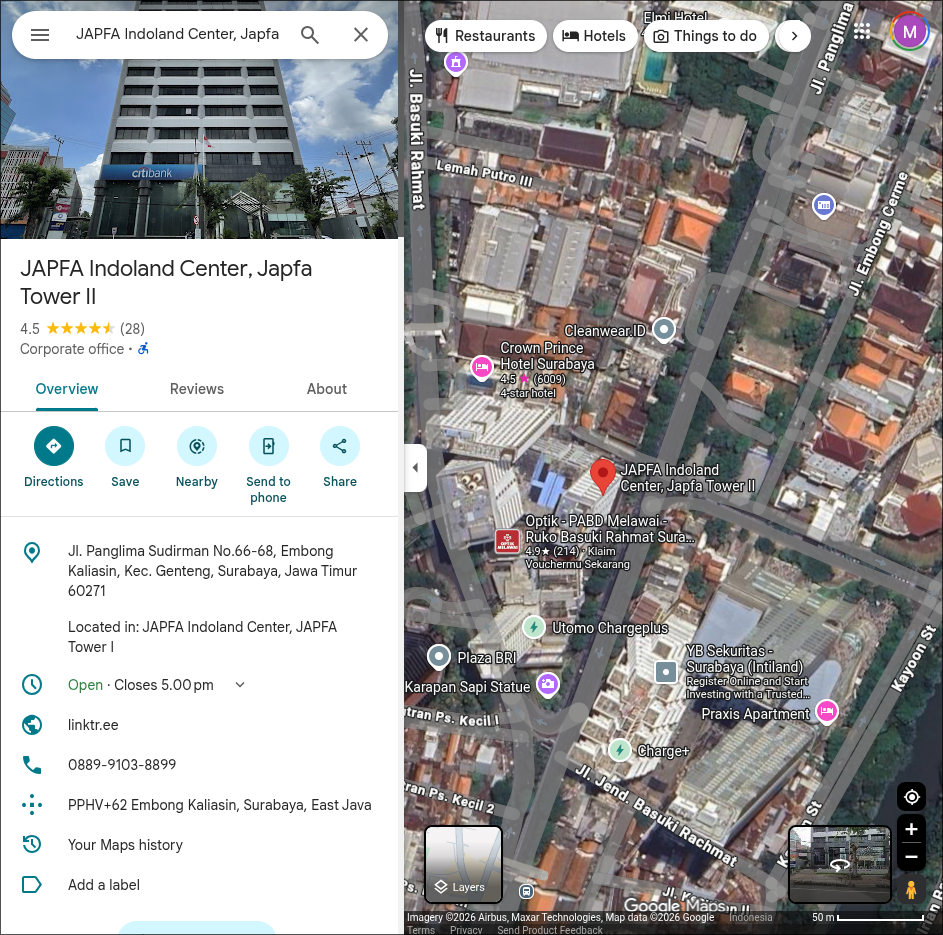
\includegraphics[width=0.55\textwidth]{assets/japfa_tower.png}
  \caption{Gedung Lokasi Kantor \NamaPerusahaan}
  \label{fig:lokasi_perusahaan}
\end{figure}

\begin{itemize}[leftmargin=*, itemsep=0pt]
  \item \textbf{Nama Perusahaan:} \NamaPerusahaan
  \item \textbf{Alamat:} \AlamatPerusahaan
  \item \textbf{Bidang Usaha:} Pengembangan perangkat lunak dan solusi teknologi informasi
\end{itemize}

\section{ETIKA PROFESI}

Etika profesi diterapkan agar pekerjaan pengembangan perangkat lunak tidak merugikan pengguna, klien, maupun rekan kerja di lingkungan perusahaan. Selama kerja praktik, penulis mengikuti ketentuan etika kerja berikut:

\begin{enumerate}[label=\arabic*., leftmargin=*, itemsep=0pt]
  \item \textbf{Kedisiplinan.} Kehadiran kerja, penyelesaian tugas, dan pelaporan kemajuan dilakukan sesuai jadwal yang disepakati bersama. Kendala yang berpotensi menghambat pekerjaan disampaikan lebih awal agar dapat ditangani secara proaktif.
  \item \textbf{Tanggung Jawab terhadap Data.} Data pelanggan, dokumen pengiriman operasional, dan kredensial layanan tidak digunakan untuk keperluan di luar pekerjaan. Data uji dipisahkan secara ketat dari data operasional produksi, serta tangkapan layar yang memuat identitas sensitif pelanggan tidak disebarkan ke publik.
\end{enumerate}
